\section{Darstellung der Ergebnisse und Auswertung}

\subsection{Darstellung der Ergebnisse}
Mit der oben beschriebenen Messmethode wurden die in Tabelle \ref{tbl_1} dargestellten Werte gemessen.
\begin{table}
\centering
\begin{tabular}{c|c}
t in s & dN/dt in 1/10s \\ 
\toprule
20	&34\\ 

40	&29\\ 

60	&32\\ 

80	&28\\ 

100	&31\\ 

120	&25\\ 

140	&28\\ 

160	&24\\ 

180	&27\\ 

200	&24\\ 

220	&32\\ 

240	&25\\ 

260	&24\\ 

280	&27\\ 
	
300	&26\\ 

320	&25\\ 

340	&27\\ 

420	&29\\ 
	
440	&29\\ 

460	&26\\ 

480	&25\\ 

500	&26\\ 

560	&26\\ 

580	&22\\ 
	
600	&25\\ 

620	&22\\ 

640	&21\\ 

660	&20\\ 

680	&23\\ 

700	&21\\ 

760	&22\\ 

780	&20\\ 

800	&24\\ 

820	&22\\ 

840	&24\\ 

860	&23\\ 

880	&22\\ 

900	&20\\ 

920	&22\\ 

940	&20\\ 

960	&21\\ 

980	&22\\ 

1000&	18\\ 

1080&	19\\ 
	
1100&	19\\ 

\multicolumn{2}{c}{\dots}\\
\end{tabular}
\begin{tabular}{c|c}
              &           \\&\\&\\&\\&\\&\\&\\&\\&\\&\\&\\&\\&\\&\\&\\&\\&\\&\\&\\&\\&\\&\\&\\&\\&\\&\\&\\&\\&\\&\\&\\&\\&\\&\\&\\&\\&\\&\\&\\&\\&\\&\\&\\&\\

\end{tabular}
\begin{tabular}{c|c} 
\multicolumn{2}{c}{\dots}\\

1120&	18\\

1160&	17\\ 

1180&	16\\ 

1200&	18\\ 

1220&	18\\ 

1240&	16	\\ 

1260&	17\\ 

1280&	15\\ 

1300&	18\\ 

1320&	16\\ 

1340&	15\\ 

1360&	14\\ 

1440&	13\\ 

1460&	12\\ 

1480&	12	\\ 

1500&	13\\ 

1520&	12\\ 

1540&	12\\ 

1560&	10	\\ 

1580&	12\\ 

1600&	12\\ 

1640&	9\\ 

1660&	8\\ 

1680&	8\\ 

1700&	8\\ 

1720&	9\\ 

1740&	8\\ 

1760&	8\\ 

1780&	8\\ 

1840&	7\\ 

1860&	6\\ 

1880&	7\\ 

1900&	6\\ 

1920&	6\\ 

1940&	6\\ 

2000&	5\\ 

2020&	5\\ 

2040&	5\\ 

2060&	5\\ 

2080&	5\\ 

2160&	5\\ 

2180&	4\\ 

2200&	4\\ 

2220&	3\\ 

\end{tabular} 
\caption{Anzahl der innerhalb von 10s durchgelaufenen Ringe in Abhängigkeit der Zeit}
\label{tbl_1}
\end{table}

\begin{figure}
\centering
        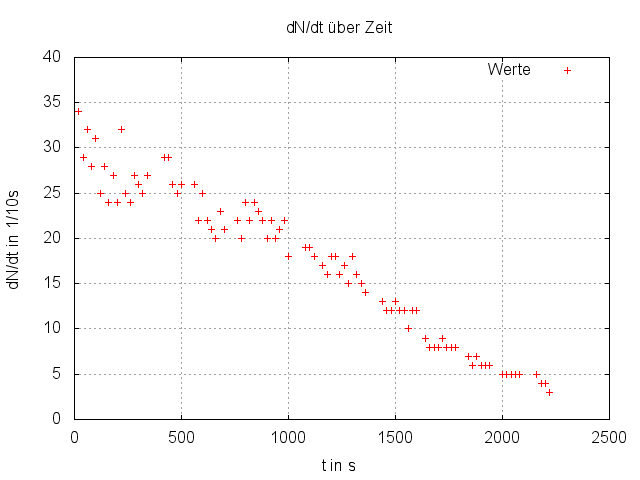
\includegraphics[width=.8\textwidth]{images/dNdt(t).png}
\caption{Anzahl der innerhalb von 10s druchgelaufenen Ringe in Abhängigkeit der Zeit}
\label{dNdt(t)}
\end{figure}


\begin{figure}
\centering
	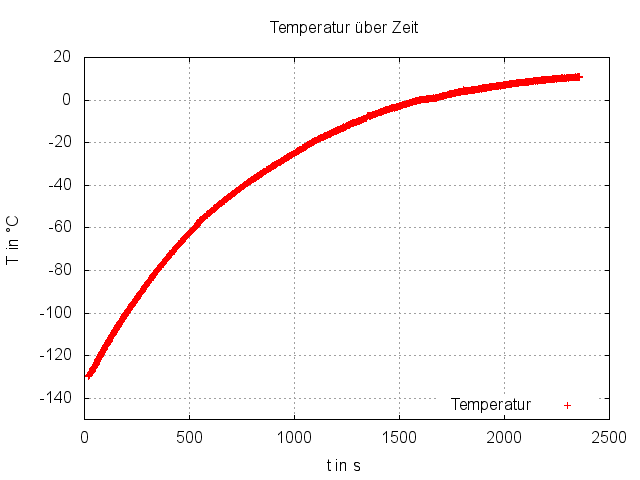
\includegraphics[width=.8\textwidth]{images/T(t).png}
\caption{Temperatur in Abhängigkeit der Zeit}
\label{plot:Tt}
\end{figure}

In Abb. \ref{dNdt(t)} wurde die Anzahl der in 10 Sekunden durchlaufenen Maxima über der Zeit aufgetragen. Der Verlauf
ist bis etwa $ t = 2000 s$ annähernd linear, danach wird der Verlauf flacher und nähert sich der Zeit-Achse an. Die Größe
$ \frac{dN}{dt} $ ist nach \eqref{form:ausdzumax} proportional zur Geschwindigkeit der Längenänderung des Stabes. In diese
Längenänderung fließt nach \eqref{form:ausdehnung} ein im Allgemeinen temperaturabhängiges $ \alpha $ sowie der zeitliche 
Verlauf der Temperaturkurve ein. Für den Temperaturverlauf ist nach \eqref{form:konvektion2} ein exponentieller Abfall
zu erwarten, aber das Verhalten von $ \alpha(T) $ ist nicht bekannt, sondern soll gerade mit diesem Versuch ermittelt werden. 
Weiter fällt sofort auf, dass die Messwerte bei großen Werten von dN/dt wesentlich
mehr streuen, was darauf zurückzuführen ist, dass das Zählen der Ringe bei größeren Werten von dN/dt mehr 
Schwierigkeiten bereitet hat.
Eine Tabelle der Temperatur des Stabes in Abhängigkeit der Zeit ist im Anhang zu finden. \\


In \aref{plot:Tt} wird der Temperaturverlauf über der Zeit aufgetragen. Der Graph steigt zu Beginn sehr schnell und nähert
sich dann der Raumtemperatur von etwa $ 20 ^{\circ} C $ an. Der Verlauf ähnelt sehr stark einer an der Zeitachse 
gespiegelten und nach oben verschobenen Exponentialfunktion, wie es nach \eqref{form:konvektion2} zu erwarten ist. 
An der Temperaturkurve ist weiter bei $ 0 ^{\circ} C $ ein kurzes Gleichbleiben der Temperatur zu beobachten. Dies ist darauf zurückzuführen, dass sich Eis um den Stab gebildet hat. Dieses schmilzt bei $ 0 ^{\circ} C $ und hält den Stab so kurzzeitig auf einer konstanten Temperatur.

\subsection{Auswertung}
Aus den gemessenen Daten kann der Wärmeausdehnungskoeffizient $ \alpha $ des verwendeten Stabes in Abhängigkeit von der Temperatur bestimmt werden. Dafür werden in dieser Auswertung zwei verschiedene Methoden verwendet und anschließend miteinander verglichen.

\subsubsection{Einteilung der Messwerte in Fraktionen}
Bei dieser Methode werden die Messwerte möglichst gleichmäßig in Fraktionen (Tabelle \ref{tbl_2}) eingeteilt und es wird jeweils innerhalb dieser der Mittelwert von $dN/dt$ gebildet.\\
(Die Mittelwertbildung ist aus mehreren Gründen gerechtfertigt: Zum Einen wird gerade ein gemittelter Wärmeausdehnungskoeffizient bestimmt. Zum anderen kann dN/dt in den Fraktionen als linear approximiert werden, wodurch sich Abweichungen vom Mittelwert durch die Linearität gegenseitig aufheben.) Außerdem werden aus den zu den Fraktionen passenden Zeitintervallen die entsprechenden Zeitdifferenzen errechnet. Aus den so bestimmten Größen kann dann für jede Fraktion ein mittlerer Wärmeausdehnungskoeffizient nach \eqref{formel:ausdehnung} folgendermaßen ermittelt werden:

\begin{equation}
\alpha(T)=\frac{\Delta L(T)}{L_{0} \cdot \Delta T}
\end{equation}

Aus $ \Delta L = \frac{\lambda}{2} \cdot \Delta N $ \eqref{form:ausdzumax_1} folgt:

\begin{equation}
\alpha (T)= \frac{\lambda}{2} \cdot \frac{\Delta N(T)}{L_0 \cdot \Delta T}
\end{equation}

\begin{table}
\centering
\begin{tabular}{ccc}

Fraktion&	Zeitintervalle in s	& $\Delta T $ in $ ^{\circ} C$ \\
\toprule
1		&[20, 180]		&26,5\\

2		&[200, 340]		&18,9\\

3		&[420, 500]		&8,7\\

4		&[560, 700]		&11,1\\

5		&[760, 880]		&7,9\\

6		&[900,1000]		&6,1\\

7		&[1080,1120]		&1,9\\

8		&[1160,1260]		&4,4\\

9		&[1280,1360]		&3,6\\

10		&[1440,1600]		&4,6\\

11		&[1640,1780]		&2,9\\

12		&[1840,1940]		&1,8\\

13		&[2000,2080]		&1,3\\

14		&[2160,2220]		&0,7\\

\end{tabular}

\caption{Einteilung in Fraktionen}
\label{tbl_2}
\end{table}



Für die Mittelwerte von $dN/dt$ mit zugehörigen Fehlern ergeben sich die in Tabelle \ref{tbl_3} dargestellten Werte.

\begin{table}
\centering
\begin{tabular}{ccc}

Fraktion	&Mittelwert von dN/dt in 1/10s	&Fehler von dN/dt in 1/10s \\
\toprule
1		&28,67				&1,08\\

2		&26,25				&0,92\\

3		&27					&0,84\\

4		&22,5				&0,73\\

5		&22,43				&0,53\\

6		&20,5				&0,62\\

7		&18,67				&0,33\\

8		&17					&0,37\\

9		&15,6				&0,68\\

10		&12					&0,29\\

11		&8,25				&0,16\\

12		&6,33				&0,21\\

13		&5					&0\\

14		&4					&0,41\\

\end{tabular}
\caption{Mittelwerte und Fehler von dN/dt}
\label{tbl_3}
\end{table}


An Tabelle \ref{tbl_3} und deren graphischen Darstellung \aref{dNdt(t)MWmitaltenWerten} fällt sofort auf, dass 
der Fehler in Fraktion 13 Null ist. Dies resultiert daraus, dass alle in dieser Fraktion zusammengefassten Werte 
gleich 5/10s sind. 


\begin{figure}
\centering
        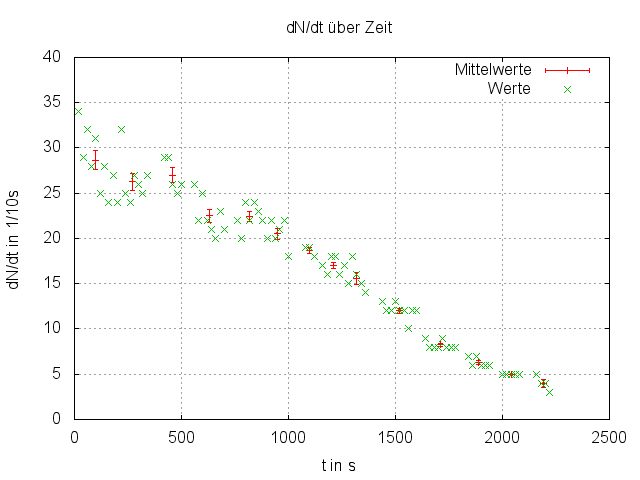
\includegraphics[width=.8\textwidth]{images/dNdt(t)MWmitaltenWerten.png}
\caption{Einteilung in Fraktionen}
\label{dNdt(t)MWmitaltenWerten}
\end{figure}


Für die Fehlerabschätzung von $ \alpha $ wird eine Fehlerfortpflanzung durchgeführt.
Dabei sind die Fehler von $ \lambda $  und  $ \Delta T $ vernachlässigbar klein. Im Fall von $ \Delta T $ ist der Fehler sogar nicht ermittelbar, da auf Grund der Benutzung von CASSY diesbezüglich keine ausreichenden Angaben vorhanden sind.

Der Fehler von $ L_{0} $ beträgt aufgrund der Messung mit einem Zollstock $ 1 mm $.

Die Fehlerfortpflanzung liefert:

\begin{equation}
\Delta (\alpha) = \frac{\lambda}{2 \cdot \Delta T} \cdot \sqrt{\frac{1}{L_{0}^{2}} \cdot (\Delta(\Delta N))^{2} + \frac{(\Delta N)^{2}}{(L_{0})^{4}} \cdot (\Delta L_{0})^{2}}
\end{equation}


Damit ergitb sich für den temperaturabhängigen Wärmeausdehnungskoeffizient der in Tabelle \ref{tbl_4} tabellarisch und in \aref{alpha(T)}
graphisch dargestellte Verlauf. Es ist eindeutig zu erkennen, dass der Ausdehnungskoeffizient mit zunehmender Temperatur 
im Bereich zwischen $ -120 $ und $ - 20 ^{\circ} C $ ebenfalls zunimmt. Es bietet sich hier ein linearer Verlauf an.
Für den Bereich ab $ -20 ^{\circ} C $ ist es aufgrund der großen Fehler schwierig, den Verlauf zu interpretieren. Grund 
dafür ist auch, dass die in einem zehnsekündigen Intervall gezählten Maxima sich im Bereich von etwa 5 bewegten. Da die
Messung nicht notwendigerweise auf ein Maximum begonnen und beendet wurde, sondern zu von der Uhr vorgegebenen Zeitpunkten,
ergibt sich hier eigentlich noch ein zusätzlicher Fehler, der für kleine $dN/dt$ relativ gesehen 
zunehmend größer wird. \\
Fittet man in \aref{alpha(T)} einen linearen Graphen, so ergibt sich die Näherung:
\begin{equation}
\alpha(T) = a \cdot T + b 
\end{equation}
mit $ a = (0,0182 \pm 0,003) \cdot 10^{-5} K^{-2} $ und $ b = (4,07 \pm 0,143) \cdot 10^{-5} K^{-1} $. Dabei wurde lediglich
der von gnuplot ausgegebene Fehler aufgeführt, aber keine erneute Fehlerfortpflanzung mit Berücksichtigung der Fehler der einzelnen
Mittelwerte durchgeführt. 

\begin{table}
\centering
\begin{tabular}{ccc}

Mittlere Temperatur in $^{\circ}C$ &$ \alpha $ in $ 10^{-5}\frac {1}{^{\circ}C} $	&Fehler von $ \alpha $ in $ 10^{-5} \frac{1}{^{\circ}C}  $ \\
\toprule
-115,6&				1,896	&		0,072\\

-90,2	&			2,129	&		0,075\\

-66,9	&			2,719	&		0,085\\

-50,1	&			3,108	&		0,101\\

-35,9	&			3,731	&		0,089\\

-27,9	&			3,680	&		0,112\\

-19,2	&			4,305	&		0,078\\

-14,0	&			4,231	&		0,093\\

-9,3	&			3,797	&		0,166\\

-2,1	&			4,571	&		0,112\\

2,1		&		4,362		&	0,086\\

5,3		&		3,851		&	0,128\\

7,7		&		3,370		&	0,011\\

9,4		&		3,755		&	0,385\\

\end{tabular}
\caption{Wärmeausdehnungskoeffizient in Abhängigkeit der Temperatur}
\label{tbl_4}
\end{table}

\begin{figure}
\centering
        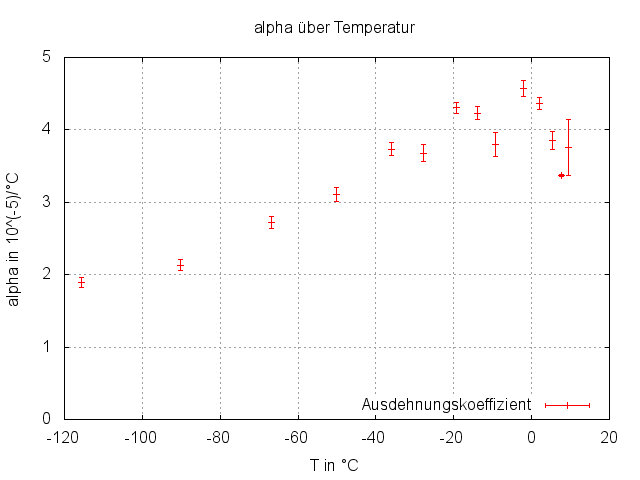
\includegraphics[width=.8\textwidth]{images/alpha(T).png}
\caption{Wärmeausdehnungskoeffizient in Abhängigkeit der Temperatur}
\label{alpha(T)}
\end{figure}


\subsubsection{Berechnung des Ausdehnungskoeffizienten durch approximatives Fitten}

Bei dieser Methode werden dN/dt und T(t) gefittet und daraus der Ausdehnungskoeffizient in Abhängigkeit der Temperatur bestimmt.

dN/dt lässt sich gut mit einem Polynom 5. Grades approximieren:


Dabei ergibt sich für 


\begin{equation}
\dot{N}(t)=a_{0}+a_{1} \cdot t+a_{2}t^{2}+a_{3}t^{3}+a_{4}t^{4}+a_{5}t^{5} :
\end{equation}

$
 a_{0} =(3,153 \pm 0,104) s^{-1} 
$

$
a_{1}=(-0,00311 \pm 0,00097)s^{-2}
$

$
a_{2}=(5,78 \pm 2,65)10^{-6}s^{-3}
$

$
a_{3}=(-5,83 \pm 2,99)10^{-9}s^{-4}
$

$
a_{4}=(2,33 \pm 1,47)10^{-12}s^{-5}
$

$
a_{5}=(-3,21 \pm 2,62)10^{-16}s^{-6} 
$\\



\begin{figure}
\centering
        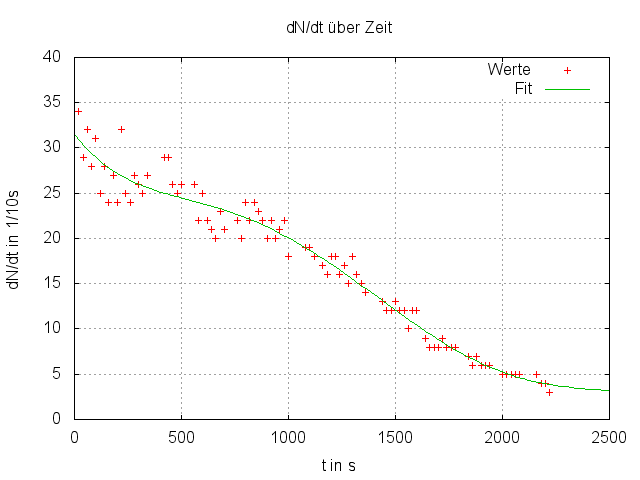
\includegraphics[width=.8\textwidth]{images/Fit_dNdt(t).png}
\caption{Fit von dN/dt}
\label{Fit dNdt(t)}
\end{figure}


T(t) lässt sich sehr gut mit einer e-Funktion approximieren:

Dabei ergibt sich für $ T(t) = a \cdot e^{bt} + c $ :

$a = (-154,01 \pm 0,04)^{\circ}C$,
$b=(-0,0012499 \pm 0,0000011)s^{-1}$,
$c=(19,91 \pm 0,042)^{\circ}C$ \\


\begin{figure}
\centering
        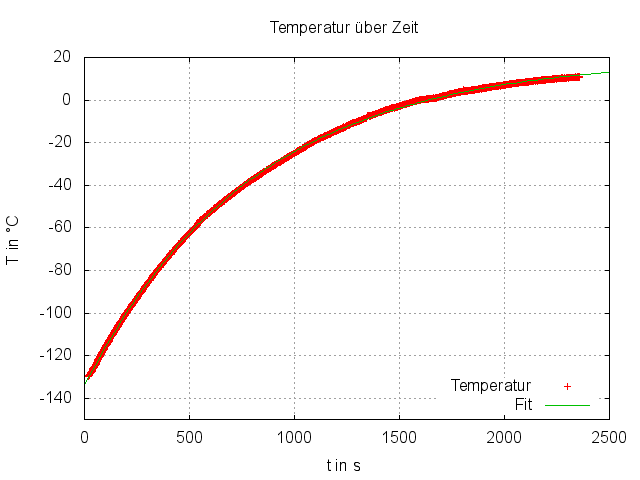
\includegraphics[width=.8\textwidth]{images/Fit_T(t).png}
\caption{Fit von T(t)}
\label{Fit T(t)}
\end{figure}


Herleitung einer Formel zur Berechnung des Ausdehnungskoeffizienten:

Wegen $ \Delta L = \alpha \cdot L_{0} \cdot \Delta T $  (nach \eqref{formel:ausdehnung}) folgt: 

\begin{equation}
\alpha (T) = \frac{1}{L_{0}} \frac{\partial L}{\partial T}
\end{equation}
Außerdem gilt: 
\begin{equation}
L = \frac{\lambda}{2} N
\end{equation}

\begin{equation}
\Rightarrow \alpha(T) = \frac{1}{L_{0}} \frac{\lambda}{2} \frac{\partial N}{\partial T} = \frac{\lambda}{2} \cdot L_{0} \frac{\partial N}{\partial t} \frac{\partial t}{\partial T}
\end{equation}

\begin{equation}
\Rightarrow \alpha (T) = \frac{\lambda}{2 \cdot L_{0}} \frac{\dot{N}(t(T))}{\dot{T}(t(T))}
\end{equation}  

Dann ergibt sich der Graph \aref{alpha(T)mitFit}


\begin{figure}
\centering
        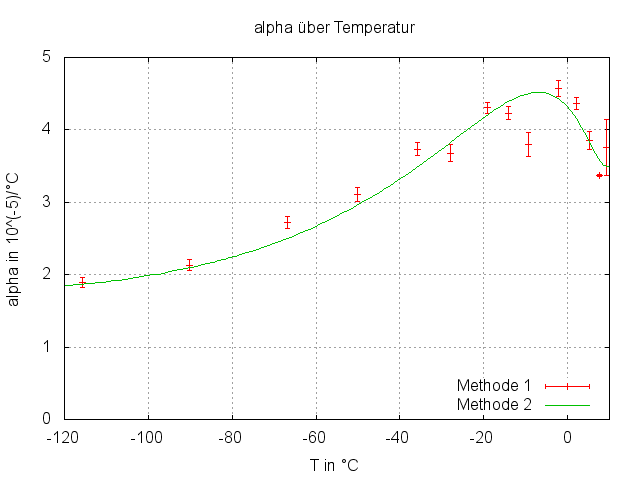
\includegraphics[width=.8\textwidth]{images/alpha(T)mitFit.png}
\caption{Vergleich zwischen Methode 1 und 2}
\label{alpha(T)mitFit}
\end{figure}


\subsubsection{Vergleich beider Methoden}
Wie in \aref{alpha(T)mitFit} zu erkennen, führen beide Methoden zu ähnlichen Ergebnissen: Im Temperaturbereich zwischen $ -120 $ und $ -20 ^{\circ} C $ stimmt der Verlauf des Graphen gut mit den Messwerten überein. Der Graph verläuft hier durch zwei von sieben und berührt zwei weitere Fehlerbalken. Im Temperaturbereich zwischen $ -20 $ und $ 10 ^{\circ} C $ stimmt der Verlauf des Graphen nur bedingt mit den Messwerten überein, da beispielweise der Messwert bei $T = -9,3 ^{\circ} C $ weit vom durch Methode 2 erlangten Graphen entfernt ist. Dies liegt vor allem daran, dass in diesem Temperaturbereich der oben schon angesprochene und nicht eingezeichnete Fehler relativ groß ist, da hier nur geringe Maximumsdurchläufe pro zehn Sekunden gezählt werden konnten.

\subsection{Fazit}


Der Bau des Interferometers hat sich als sehr schwierig herrausgestellt, da die Spiegel sehr genau ausgerichtet sein müssen.
Weitere Probleme sind bei der Messung der Ausdehnung des Stabs entstanden. Der vom Stab geschobene Spiegel musste so auf einer Schiene befestigt sein, dass er sich dabei nicht verdreht.
Durch das Zählen von Interferenzringen konnten dennoch Messungen durchgeführt werden, welche damit die Funktionstüchtigkeit des Michelson-Interferometers bestätigten.


